%%%%%%%%%%%%%%%%%%%%%%%%%%%%% Define Article %%%%%%%%%%%%%%%%%%%%%%%%%%%%%%%%%%
\documentclass{article}
%%%%%%%%%%%%%%%%%%%%%%%%%%%%%%%%%%%%%%%%%%%%%%%%%%%%%%%%%%%%%%%%%%%%%%%%%%%%%%%

%%%%%%%%%%%%%%%%%%%%%%%%%%%%% Using Packages %%%%%%%%%%%%%%%%%%%%%%%%%%%%%%%%%%
\usepackage{geometry}
\usepackage{graphicx}
\usepackage{amssymb}
\usepackage{amsmath}
\usepackage{amsthm}
\usepackage{empheq}
\usepackage{mdframed}
\usepackage{booktabs}
\usepackage{lipsum}
\usepackage{graphicx}
\usepackage{color}
\usepackage{psfrag}
\usepackage{pgfplots}
\usepackage{bm}
\usepackage[version=4]{mhchem}
\usepackage{chemformula}
%%%%%%%%%%%%%%%%%%%%%%%%%%%%%%%%%%%%%%%%%%%%%%%%%%%%%%%%%%%%%%%%%%%%%%%%%%%%%%%

% Other Settings

%%%%%%%%%%%%%%%%%%%%%%%%%% Page Setting %%%%%%%%%%%%%%%%%%%%%%%%%%%%%%%%%%%%%%%
\geometry{a4paper}

%%%%%%%%%%%%%%%%%%%%%%%%%% Define some useful colors %%%%%%%%%%%%%%%%%%%%%%%%%%
\definecolor{ocre}{RGB}{243,102,25}
\definecolor{mygray}{RGB}{243,243,244}
\definecolor{deepGreen}{RGB}{26,111,0}
\definecolor{shallowGreen}{RGB}{235,255,255}
\definecolor{deepBlue}{RGB}{61,124,222}
\definecolor{shallowBlue}{RGB}{235,249,255}
%%%%%%%%%%%%%%%%%%%%%%%%%%%%%%%%%%%%%%%%%%%%%%%%%%%%%%%%%%%%%%%%%%%%%%%%%%%%%%%

%%%%%%%%%%%%%%%%%%%%%%%%%% Define an orangebox command %%%%%%%%%%%%%%%%%%%%%%%%
\newcommand\orangebox[1]{\fcolorbox{ocre}{mygray}{\hspace{1em}#1\hspace{1em}}}
%%%%%%%%%%%%%%%%%%%%%%%%%%%%%%%%%%%%%%%%%%%%%%%%%%%%%%%%%%%%%%%%%%%%%%%%%%%%%%%

%%%%%%%%%%%%%%%%%%%%%%%%%%%% English Environments %%%%%%%%%%%%%%%%%%%%%%%%%%%%%
\newtheoremstyle{mytheoremstyle}{3pt}{3pt}{\normalfont}{0cm}{\rmfamily\bfseries}{}{1em}{{\color{black}\thmname{#1}~\thmnumber{#2}}\thmnote{\,--\,#3}}
\newtheoremstyle{myproblemstyle}{3pt}{3pt}{\normalfont}{0cm}{\rmfamily\bfseries}{}{1em}{{\color{black}\thmname{#1}~\thmnumber{#2}}\thmnote{\,--\,#3}}
\theoremstyle{mytheoremstyle}
\newmdtheoremenv[linewidth=1pt,backgroundcolor=shallowGreen,linecolor=deepGreen,leftmargin=0pt,innerleftmargin=20pt,innerrightmargin=20pt,]{theorem}{Theorem}[section]
\theoremstyle{mytheoremstyle}
\newmdtheoremenv[linewidth=1pt,backgroundcolor=shallowBlue,linecolor=deepBlue,leftmargin=0pt,innerleftmargin=20pt,innerrightmargin=20pt,]{definition}{Definition}[section]
\theoremstyle{myproblemstyle}
\newmdtheoremenv[linecolor=black,leftmargin=0pt,innerleftmargin=10pt,innerrightmargin=10pt,]{problem}{Problem}[section]
%%%%%%%%%%%%%%%%%%%%%%%%%%%%%%%%%%%%%%%%%%%%%%%%%%%%%%%%%%%%%%%%%%%%%%%%%%%%%%%

%%%%%%%%%%%%%%%%%%%%%%%%%%%%%%% Plotting Settings %%%%%%%%%%%%%%%%%%%%%%%%%%%%%
\usepgfplotslibrary{colorbrewer}
\pgfplotsset{width=8cm,compat=1.9}
%%%%%%%%%%%%%%%%%%%%%%%%%%%%%%%%%%%%%%%%%%%%%%%%%%%%%%%%%%%%%%%%%%%%%%%%%%%%%%%

%%%%%%%%%%%%%%%%%%%%%%%%%%%%%%% Title & Author %%%%%%%%%%%%%%%%%%%%%%%%%%%%%%%%
\title{9701 Chemistry Theory — Transition Metals}
\author{Alston}
\date{}
\parskip=3pt
\parindent=0pt
%%%%%%%%%%%%%%%%%%%%%%%%%%%%%%%%%%%%%%%%%%%%%%%%%%%%%%%%%%%%%%%%%%%%%%%%%%%%%%%

\begin{document}
    \maketitle
    \section{Introduction}
    My compiled notes for the transition metal section of the CAIE 9701 Chemistry course.

    \section{Transition Element Basics}
    \begin{definition}[Transition Element]
        A transition element is a d-block element that forms one or more stable ions with an incomplete d subshell.
    \end{definition}

    Notice that Scandium ($\ce{Sc}$) and Zinc ($\ce{Zn}$) are therefore $\textbf{NOT}$ transition elements.

    The variable oxidation states of the transition elements comes from the similar energy in the $3d$ and $4s$ orbitals, so there are many options of number of electrons to remove to end up at a stable ion.

    For the transition metals, as they go across the row, the most common oxidation state becomes $+2$. This is due to the fact that the $3d$ sub electrons are more stable. 

    \subsection{Cause of Colour}
    When ligands are attached to a transition element, the d-orbitals are split into two non-degenerate orbitals of different energy levels. Electrons absorb energy to jump up the orbital, and when they come down they release the excess energy in the form of light. The $d_{x^2 - y^2}$ and $d_{z^2}$ orbitals have different energy than the other 3.
    \begin{center}
        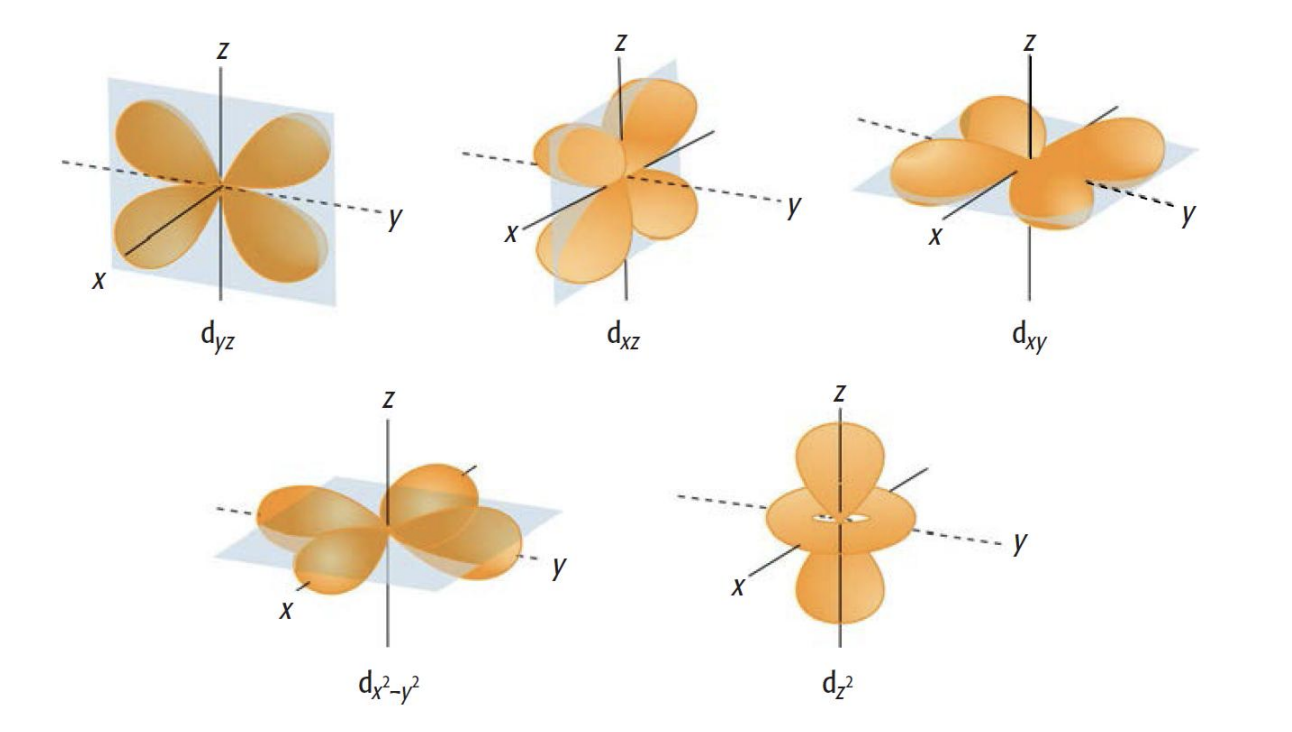
\includegraphics[width=0.6\textwidth]{image.png}
    \end{center}
    \begin{center}
        $\textit{5 different arrangements of d-orbitals.}$
    \end{center}

    \section{Complex Ion Formation}
    \begin{definition}[Ligands]
        A species that contains a lone pair of electrons that forms a dative (coordinate) bond with a central transition element.
    \end{definition}

    \begin{definition}[Complex Ion]
        A complex ion is an ion formed by a central transition element surrounded by one or more ligands.
    \end{definition}

    \begin{definition}[Coordination Number]
        A coordination number of a complex ion is the number of dative bonds to the central transition element.
    \end{definition}

    \subsection{Isomerism}
    Complex ions can form geometric or optical isomers. Generally, optical isomers happen when a transition element is bonded to 3 bidentate ligands. The Cis-Trans isomers happen when there are more than one type of ligands bonded to a central atom.


    \section{Reactions: Redox and Ligand Exchange}

    \begin{center}
        \begin{tabular}{|l|l|l|}
            \hline
            \multicolumn{3}{|c|}{\textbf{Copper (Cu)}} \\
            \hline
            [Cu(H$_2$O)$_6$]$^{2+}$ & Blue & Octahedral \\
            \ce{[Cu(H2O)4(OH)2]} & Blue ppt & Octahedral \\
            \ce{[CuCl4]^2-} & Yellow/green & Tetrahedral \\
            \ce{[Cu(NH3)4(H2O)2]^2+} & Deep blue & Square planar/dist. octahedral \\
            \hline
            \multicolumn{3}{|c|}{\textbf{Cobalt (Co)}} \\
            \hline
            [Co(H$_2$O)$_6$]$^{2+}$ & Pink & Octahedral \\
            \ce{[CoCl4]^2-} & Blue & Tetrahedral \\
            \ce{[Co(NH3)6]^2+} & Brown/ & Octahedral \\
            \hline
            \multicolumn{3}{|c|}{\textbf{Nickel (Ni)}} \\
            \hline
            [Ni(H$_2$O)$_6$]$^{2+}$ & Green & Octahedral \\
            \ce{[Ni(NH3)6]^2+} & Violet & Octahedral \\
            \ce{[Ni(CN)4]^2-} & Colourless & Square planar \\
            \hline
            \multicolumn{3}{|c|}{\textbf{Iron (Fe)}} \\
            \hline
            [Fe(H$_2$O)$_6$]$^{2+}$ & Pale green & Octahedral \\
            \ce{[Fe(H2O)6]^3+} & Yellow-brown & Octahedral \\
            \hline
            \multicolumn{3}{|c|}{\textbf{Chromium (Cr)}} \\
            \hline
            [Cr(NH$_3$)$_6$]$^{3+}$ & Purple & Octahedral \\
            \hline
        \end{tabular}
    \end{center}
    
    \section{Stability Constants}
    $K_{stab}$ is just another form of an equilibrium constant and it's calculated in the same way as the other ones. The higher a $K_{stab}$ is, the more stable the complex ion.

    


\end{document}